%%==================================================
%% chapter03.tex for BIT Master Thesis
%% modified by yang yating
%% version: 0.1
%% last update: Dec 25th, 2016

%% modified by Meng Chao
%% version: 0.2
%% last update: May 29th, 2017
%%==================================================
\chapter{单目SLAM算法研究}
\label{chap:ALGORITHM}

同步定位与地图重建(SLAM)利用多视图几何原理\upcite{[1.1]},根据图像信息估计相机在陌生环境中的位姿,构建环境地图。如果在获取图像信息时,仅使用一个摄像头,则称为单目SLAM。本章主要介绍经典视觉SLAM算法框架,研究基于该框架的两种主流单目SLAM算法,在相同数据集上对比分析两种算法的优缺点,结合无人机运动特性选择合适的SLAM算法应用于无人机导航定位。

%3.1
\section{经典视觉SLAM算法框架}
视觉SLAM实际是状态估计问题,将传感器数据抽象为适于估计的状态变量,通过运动模型与观测模型估计系统状态。经典视觉SLAM算法框架\upcite{[3.1]}一般包括3个部分:视觉里程计,后端优化和闭环检测。视觉里程计估计帧间运动和局部地图,把传感器数据抽象为适于估计的状态变量;后端优化则处理视觉里程计估计的不同时刻位姿和回环检测信息,根据观测模型和运动模型建立约束关系,估计优化相机位姿与地图点位置,得到全局一致的轨迹与地图;回环检测判断相机是否到达曾经经过的位置,如果检测到回环反馈给后端进行优化处理,视觉SLAM算法结构如图\ref{fig3.1}所示。

\begin{figure}[h]
\centering
\includegraphics[scale=0.3,angle=-90]{figures/Fig3-1.pdf}
\caption{视觉SLAM算法结构}
\label{fig3.1}
\end{figure}

%3.1.1
\subsection{视觉里程计}
视觉SLAM是一个状态估计问题,然而实际的传感器输出大都很难直接作为状态估计模型的输入。因而视觉里程计的主要任务是根据传感器输入,将图像数据抽象为适于估计的状态,根据图像得到$I_i \rightarrow I_j$的相对位姿$T_{ij}$,串联相对位姿并三角化观测到的路标点得到运动轨迹与局部地图。视觉里程计只估计相邻时刻的运动,与之前的状态没有关联。视觉里程计主要包括两个部分,传感器数据关联和运动估计\upcite{[1.39]},其算法流程如图\ref{fig3.2}所示。根据视觉里程计传感器关联数据方式的不同,将视觉SLAM分为基于直接法和基于特征的SLAM算法,具体原理将在3.2节中详细介绍。

\begin{figure}[h]
\centering
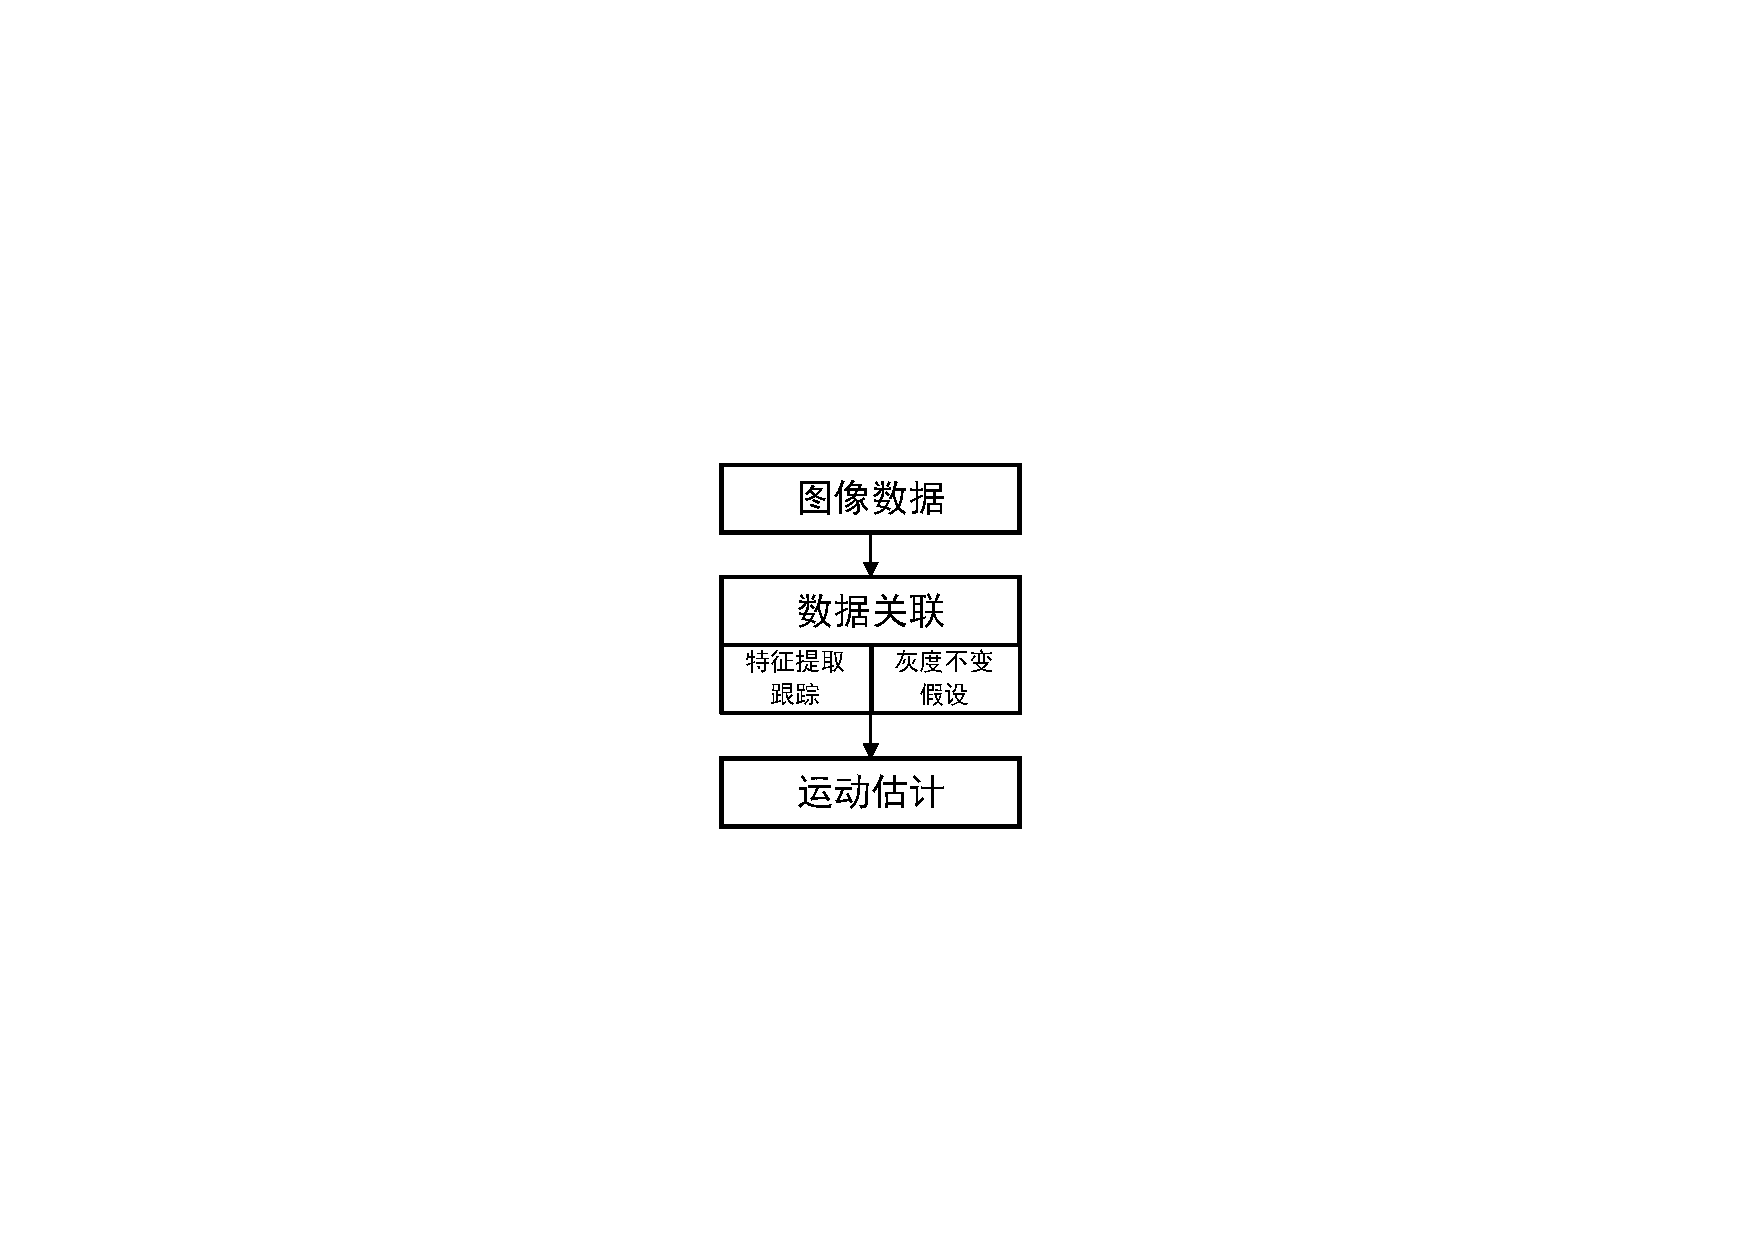
\includegraphics[scale=0.7,angle=-90]{figures/Fig3-2.pdf}
\caption{视觉里程计算法流程图}
\label{fig3.2}
\end{figure}
\vspace{-20pt}

视觉里程计得到的轨迹和地图,由于在运动估计时只考虑了帧间的信息,每次估计都带有一定的误差,串联的轨迹无可避免会出现累计漂移,这将导致无法得到全局一致的轨迹与地图。需要通过后端优化算法进行处理,估计运动和周围环境的不确定性,减小误差,提高轨迹和地图的精度。


%3.1.2
\subsection{后端优化}
SLAM后端优化将SLAM看作最大后验估计问题,且大都采用因子图的方式来表示变量之间的依赖关系\upcite{[3.2]}。一般的,假设状态变量为$\mathcal{X}$,变量$\mathcal{X}$包括无人机的轨迹和地图点的位置。传感器的测量值$Z=\lbrace z_k:k=1,\ldots ,m\rbrace$,且每个测量值可以表示为状态变量$\mathcal{X}$的函数,例如$z_k=h_k\left( \mathcal{X}_k \right)+\epsilon_k$,其中$\mathcal{X}_k \in \mathcal{X}$是$k$时刻的状态变量,$h_k(\cdot)$表示传感器的观测模型,$\epsilon_k$是随机观测误差。

最大后验估计通过计算后验概率$\mathds{P}\left(\mathcal{X} \vert Z\right)$取最大时对应的变量$\mathcal{X}^*$来估计状态变量$\mathcal{X}$的值
\begin{equation}
\label{equ3.1}
\mathcal{X}^* 
\doteq 
\argmax \limits_{\mathcal{X}} \mathds{P}\left(\mathcal{X} \vert Z\right) 
=
\argmax \limits_{\mathcal{X}}\mathds{P}\left(Z \vert \mathcal{X}  \right)\mathds{P}\left(\mathcal{X}\right)
\end{equation}
在公式\eqref{equ3.1}中$\mathds{P}\left(Z \vert \mathcal{X}  \right)$表示在状态变量$\mathcal{X}$确定情况下测量值$Z$的似然,$\mathds{P}\left(\mathcal{X}\right)$表示状态$\mathcal{X}$的先验概率。先验概率包括任何关于状态$\mathcal{X}$的先验信息,如果没有可用的先验信息,则$\mathds{P}\left(\mathcal{X}\right)$表示为一个常量,可以从优化过程中移除。在这种情况下,最大后验估计可以简化为极大似然估计。

假设测量值$Z=\lbrace z_k:k=1,\ldots ,m\rbrace$相互独立(测量噪声不相关),公式\eqref{equ3.1}可以表示为:
\begin{equation}
\label{equ3.2}
\mathcal{X}^* 
= 
\argmax \limits_{\mathcal{X}} \mathds{P}\left(\mathcal{X}\right) \prod \limits_{k=1}^{m} \mathds{P}\left(z_k \vert \mathcal{X}  \right)
=
\mathds{P}\left(\mathcal{X}\right) \prod \limits_{k=1}^{m} \mathds{P}\left(z_k \vert \mathcal{X}_k  \right)
\end{equation}
其中,等式右边的测量值$z_k$仅仅与状态变量$\mathcal{X}_k$有关。

公式\eqref{equ3.2}可以用因子图\upcite{[3.3]}表示,如图\ref{fig3.3}所示。状态变量作为节点(图中的$x_i,l_i,K$),似然$\mathds{P}\left(z_k \vert \mathcal{X}_k  \right)$和先验$\mathds{P}\left(\mathcal{X} \right)$作为因子(图中的黑色方框),描述了对节点的概率约束。因子图表示了第$k$个因子和对应状态变量$\mathcal{X}_k$依赖关系的图模型。因子图将SLAM问题可视化,便于理解。

\begin{figure}[h]
\centering
\includegraphics[scale=0.5,angle=-90]{figures/Fig3-3.pdf}
\caption{SLAM因子图}
\label{fig3.3}
\end{figure}
\vspace{-20pt}

为了更清楚的表示公式\eqref{equ3.2},假设观测模型的测量噪声$\epsilon_k$服从信息矩阵为$\Omega_k$的零偏高斯分布。测量值的似然可以表示为
\begin{equation}
\label{equ3.3}
\mathds{P}\left(z_k \vert \mathcal{X}_k  \right) \varpropto \exp ( -{1 \over 2} \left\| z_k -  h_k\left( \mathcal{X}_k \right) \right\|_{\Omega_k}^2 )
\end{equation}
其中$\left\| e \right\|_{\Omega}^2 = e^T \Omega e$。类似的,假设先验也服从高斯分布:
\begin{equation}
\label{equ3.4}
\mathds{P}\left( \mathcal{X}  \right) \varpropto \exp ( -{1 \over 2} \left\| z_0 - h_0\left(  \mathcal{X} \right)  \right\|_{\Omega_0}^2 )
\end{equation}
其中$h_0(\cdot)$表示观测模型,先验均值为$z_0$,信息矩阵为$\Omega_0$。由于最大后验与最小负对数后验等价,则公式\eqref{equ3.2}的最大后验估计可以表示为:
\begin{equation}
\label{equ3.5}
\mathcal{X}^* 
=
\argmin \limits_{\mathcal{X}} - \log \left( \mathds{P}\left(\mathcal{X}\right) \prod \limits_{k=1}^{m} \mathds{P}\left(z_k \vert \mathcal{X}_k  \right) \right)
=
\argmin \limits_{\mathcal{X}} \sum \limits_{k=0}^{m} -{1 \over 2} \left\|  z_k - h_k\left(   \mathcal{X}_k \right)  \right\|_{\Omega_k}^2
\end{equation}
公式\eqref{equ3.5}的形式是典型的非线性最小二乘问题,其中$h_k(\cdot)$是一个非线性函数。需要注意,公式\eqref{equ3.5}的前提是假设观测模型的观测噪声服从高斯分布,对于不同的观测噪声分布,将会得到不同的目标优化函数。例如,若观测噪声服从拉普拉斯分布,则公式\eqref{equ3.5}的平方$l_2$范数应变为$l_1$范数。另外,为了增加算法对于离群值的鲁棒性,通常使用鲁棒核函数\upcite{[3.4]}替换公式\eqref{equ3.5}中的平方$l_2$范数。

公式\eqref{equ3.5}的形式与SFM中的Bundle Adjustment(BA)问题相似,这是因为公式\eqref{equ3.5}与BA都是从最大后验估计出发推导得到的。但是,SLAM问题具有两个特点。首先,不同于SFM中的BA问题受限于几何模型约束,公式\eqref{equ3.5}适用于各种传感器模型。比如惯性传感器,GPS,轮式传感器等。其次,公式\eqref{equ3.5}是增量式的求解。

对于解决公式\eqref{equ3.5}的最小化问题,可通过连续线性化求解。例如高斯-牛顿法(G-N)和列文伯格-马夸尔特法(L-M)。高斯-牛顿方法从给定的初值$\hat{\mathcal{X}}$开始迭代,每次迭代时高斯-牛顿法估计公式\eqref{equ3.5}的最小值对应的状态增量
\begin{equation}
\label{equ3.6}
\delta_\mathcal{X}^* 
=
\argmin \limits_{\delta_\mathcal{X}} {1 \over 2} \sum \limits_{k=0}^{m} \left\| A_k\delta_\mathcal{X}-b_k \right\|_{\Omega_k}^2
=
\argmin \limits_{\delta_\mathcal{X}} {1 \over 2} \left\| A\delta_\mathcal{X}-b \right\|_{\Omega}^2
\end{equation}
其中公式\eqref{equ3.6}中的$\delta_\mathcal{X}$表示初始估计状态$\hat{\mathcal{X}}$的微小修正量;$A_k \doteq - {\partial h_k(\mathcal{X}) \over \partial \mathcal{X}} $是观测模型$h_k(\cdot)$关于$\mathcal{X}$的雅各比,$b_k \doteq z_k-h(\mathcal{X})$表示测量值与观测模型预测值之间的残差;公式\eqref{equ3.6}右边的矩阵$A$,$b$是由$A_k$,$b_k$组成的矩阵;$\Omega$是由观测噪声信息矩阵$\Omega_k$组成的对角块矩阵。

公式\eqref{equ3.6}对应的微小修正$\delta_\mathcal{X}^* $可以用下面的公式计算
\begin{equation}
\label{equ3.7}
\delta_\mathcal{X}^* = - \left( A^T \Omega^{-1} A \right)^{-1} A^T \Omega^{-1} b
\end{equation}
每次通过$\hat{\mathcal{X}} \leftarrow \hat{\mathcal{X}}+\delta_\mathcal{X}^*$迭代更新估计状态,矩阵$A^T \Omega^{-1} A$近似认为是Hessian矩阵。之前的推导过程中,我们假设$\mathcal{X}$属于向量空间。如果$\mathcal{X}$属于流形空间(如旋转矩阵),则高斯-牛顿法的形式保持不变,但是迭代更新方程$\hat{\mathcal{X}} \leftarrow \hat{\mathcal{X}}+\delta_\mathcal{X}$会被更合适的映射法则\upcite{[3.5]}取代。在机器人领域中,通常使用符号$\oplus$表示状态更新的映射关系,并且将状态的微小修正量$\delta_\mathcal{X}$定义在流形的切空间上,此时的更新方程为$\hat{\mathcal{X}}  \leftarrow \hat{\mathcal{X}} \oplus \delta_\mathcal{X}$。

现代SLAM算法最大的进步,在于认识到公式\eqref{equ3.7}中的雅各比矩阵$A$的稀疏性,而矩阵$A$的稀疏性是由于因子图内在的拓扑逻辑所决定的,利用矩阵稀疏性可以快速求解线性方程中状态的微小增量$\delta_\mathcal{X}^*$。此外,还可以设计增量式的求解方法,将更新后的状态变量作为新的观测值。当前主流SLAM后端优化库(如GTSAM,g2o,Ceres,iSAM,SLAM++)可以在几秒之内求解数以万计的状态变量。


%3.1.3
\subsection{回环检测}
上文介绍了SLAM的前端视觉里程计和后端优化:前端将传感器观测到的数据进行关联并将观测值抽象为适于后端估计的状态(轨迹,地图点位置);后端负责根据前端的结果对系统状态进行优化。然而,前端的视觉里程计只考虑时间关联性,之前测量产生的误差不可避免的会累计到下一时刻,产生累计误差,无法构建全局一致的轨迹和地图。后端优化虽然能够估计最大后验误差,但由于前端只提供了相邻时刻关键帧数据,无法消除累计误差。回环检测又称闭环检测,负责检测传感器是否经过同一个位置,通过增加与之前时刻的数据关联性约束,消除SLAM的轨迹与地图随时间漂移而产生的累计误差。回环检测对于SLAM算法意义重大,关系到SLAM算法估计的轨迹和地图在长时间运行中的准确性。另外,由于回环检测可以提供当前数据与历史数据的关联性,当SLAM算法前端跟踪丢失后,可以利用回环检测进行重定位,有效提高SLAM的精度和鲁棒性。

常用的回环检测方法有两种\upcite{[3.7]}:基于里程计的几何方法和基于外观的图像相似性。基于里程计的几何方法利用视觉里程计的位置信息,当发现运动到之前的某个位置附近时检测是否有回环关系。这是一种很直接的检测思路,但是由于存在累计误差,里程计无法正确的发现到底是否回到了曾经的某个位置。另一种方法是基于图像外观,这种方法和前端后端的输出无关,仅仅根据两幅图像之间的相似性进行判断。这种方法与累计误差完全无关,可以独立作为SLAM算法的一个模块,成为视觉SLAM中闭环检测的主流方法,应用于实际的SLAM系统中。


%3.2
\section{主流单目视觉SLAM算法研究}
近些年出现了许多优秀的单目SLAM算法,按照前端视觉里程计关联数据的方式不同分为基于直接法的SLAM和基于特征的SLAM两种。基于直接法的SLAM算法假设同一空间点的像素灰度值在不同图像中固定不变,估计最优位姿使得两幅图像经变换后灰度变化最小,完成前端的数据关联。基于特征的SLAM算法则提取图像中的特征,并在不同图像中对相同特征进行匹配,从而解算图像之间的相对运动,关联前端数据。本节主要研究两种代表性的单目SLAM算法:基于直接法的LSD-SLAM和基于特征的ORB-SLAM,分析对比两算法的原理、优势和不足,选择适用于无人机导航定位的单目SLAM算法,并针对其中存在的不足提出改进建议。

%3.2.1
\subsection{基于直接法的LSD-SLAM}

\subsubsection{算法概述}
LSD-SLAM是2014年慕尼黑工业大学的J.Engle等人提出的基于直接法的SLAM算法,无需计算图像特征点,通过直接法的像素关联估计运动状态,构建半稠密地图——半稠密是指估计灰度梯度明显区域的像素位置。该算法可以在大尺度环境下实时运行,利用半稠密像素关联和关键帧pose图优化构建全局一致的地图,关键帧间的pose图使用相似变换$\mathfrak{sim}(3)$代替$\mathfrak{se}(3)$,从而在后端优化中可以考虑不同场景的尺度变化,减小尺度漂移。LSD-SLAM的算法流程\upcite{[1.21]}如图\ref{fig3.4}所示。

\begin{figure}[h]
\centering
\includegraphics[scale=0.5,angle=-90]{figures/Fig3-4.pdf}
\caption{LSD-SLAM算法流程图}
\label{fig3.4}
\end{figure}
\vspace{-20pt}

LSD-SLAM算法主要分为三个部分:图像跟踪,深度估计和地图优化。图像跟踪部分获取相机采集的图像,利用上一帧的图像位姿作为初值,估计当前帧与关键帧的相对位姿$\xi \in \mathfrak{se}(3) $;深度估计部分根据当前帧情况,进行关键帧替换或位姿和像素逆深度优化。如果相机运动过快,则将新关键帧的地图点投影到临近关键帧进行初始化;如果当前帧被创建为新的关键帧,则之前关键帧的像素逆深度不再被优化。地图优化部分将之前的关键帧加入到全局地图中,使用尺度感知和图像相似变换关联来检测回环和尺度漂移,估计相邻关键帧之间的相似变换$\xi \in \mathfrak{sim}(3)$,优化关键帧的位姿和像素逆深度。

\subsubsection{数据关联与运动估计}
基于直接法的SLAM前提是灰度不变假设,即认为同一空间点的像素灰度值在不同图像中保持不变。直接法预先不知道像素之间的对应关系,而是通过最小化灰度误差来求解位姿变换和对应关系。如图\ref{fig3.5}所示,空间点$\boldsymbol{P}$的世界坐标为$[X,Y,Z]^T$,相机内参为$\boldsymbol{K}$,空间点$\boldsymbol{P}$在两幅图像中的对应像素坐标为$\boldsymbol{p_1},\boldsymbol{p_2}$。为了估计从图像1到图像2的相对位姿,以图像1的相机坐标系为参考系,假设图像2的位姿为$\boldsymbol{R},\boldsymbol{t}$,对应的李代数为$\boldsymbol{\xi} \in \mathfrak{se}(3) $。根据相机投影模型有:
\begin{equation}
\label{equ3.8}
\begin{aligned}
& \boldsymbol{p_1} = 
\begin{bmatrix}
u_1 \cr v_1 \cr 1 \cr 
\end{bmatrix}
={1 \over Z_1} \boldsymbol{K} \boldsymbol{P}
\\
& \boldsymbol{p_2} = 
\begin{bmatrix}
u_2 \cr v_2 \cr 1 \cr
\end{bmatrix}
={1 \over Z_2} \boldsymbol{K} ( \boldsymbol{R} \boldsymbol{P}+\boldsymbol{t}) = {1 \over Z_2} \boldsymbol{K} ( \exp (\boldsymbol{\xi}^{\wedge}) \boldsymbol{P})_{1:3}
\end{aligned}
\end{equation}
其中$Z_1$,$Z_2$是空间点$\boldsymbol{P}$在两个相机坐标系下的深度,$(\cdot)^{\wedge}$表示向量的反对称矩阵。由于位姿$\exp(\boldsymbol{\xi}^{\wedge})$与齐次坐标相乘,得到的结果只取前三个元素。

\begin{figure}[h]
\centering
\includegraphics[scale=0.3,angle=-90]{figures/Fig3-5.pdf}
\caption{直接法示意图}
\label{fig3.5}
\end{figure}
\vspace{-20pt}

直接法中只已知像素的灰度值,无法直接提供两幅图像的像素匹配,而是根据灰度不变假设估计相机间的相对位姿,最小化两幅图像像素灰度误差,也就是$P$点对应两个像素点的灰度误差。
\begin{equation}
\label{equ3.9}
\begin{aligned}
& e = I_1(\boldsymbol{p}_1) - I_2(\boldsymbol{p}_2) 
\\ 
& \min\limits_{\boldsymbol{\xi}} J(\boldsymbol{\xi}) = \Vert e \Vert ^2
\end{aligned}
\end{equation}
其中$I(\cdot)$表示图像像素灰度函数,目标优化函数为误差的二范数。对于空间中所有空间点,都应该满足灰度不变假设。若存在$N$个空间点$\boldsymbol{P}_i$,相机位姿估计问题可以表示为:
\begin{equation}
\label{equ3.10}
\min\limits_{\boldsymbol{\xi}} J(\boldsymbol{\xi}) = \sum\limits_{i=1}^N e_i^T e_i
\end{equation}
其中优化变量是相机位姿$\boldsymbol{\xi}$,为了得到最优解需要研究位姿$\boldsymbol{\xi}$变化对误差$e$的影响,即误差关于位姿的导数。使用李代数左乘扰动模型增加扰动$\exp( \delta \boldsymbol{\xi}^{\wedge})$,有:
\begin{equation}
\label{equ3.11}
\begin{aligned}
e(\boldsymbol{\xi}\oplus \delta \boldsymbol{\xi}) & = I_1\left({1 \over Z_1} \boldsymbol{K} \boldsymbol{P} \right) - I_2\left({1 \over Z_2} \boldsymbol{K} \exp (\delta \boldsymbol{\xi}^{\wedge}) \exp (\boldsymbol{\xi}^{\wedge}) \boldsymbol{P} \right)
\\
& \approx I_1\left( {1 \over Z_1} \boldsymbol{K} \boldsymbol{P} \right) - I_2 \left( {1 \over Z_2} \boldsymbol{K} (1+\delta \boldsymbol{\xi}^{\wedge}) \exp (\boldsymbol{\xi}^{\wedge}) \boldsymbol{P} \right)
\\
& = I_1\left( {1 \over Z_1} \boldsymbol{K} \boldsymbol{P} \right) - I_2 \left({1 \over Z_2} \boldsymbol{K} \exp (\boldsymbol{\xi}^{\wedge}) \boldsymbol{P}+ {1 \over Z_2} \boldsymbol{K} \delta \boldsymbol{\xi}^{\wedge} \exp (\boldsymbol{\xi}^{\wedge}) \boldsymbol{P} \right)
\end{aligned}
\end{equation}
记公式\eqref{equ3.11}中的$\boldsymbol{q} = \delta \boldsymbol{\xi}^{\wedge} \exp (\boldsymbol{\xi}^{\wedge}) \boldsymbol{P} $,$\boldsymbol{u}={1 \over Z_2} \boldsymbol{K} \boldsymbol{q}$,$\boldsymbol{q}$为$\boldsymbol{P}$点受到扰动后在图像2的相机坐标系下的坐标,$\boldsymbol{u}$为它的像素坐标。利用一阶泰勒近似,得到:
\begin{equation}
\label{equ3.12}
\begin{aligned}
e(\boldsymbol{\xi}\oplus \delta \boldsymbol{\xi}) &= I_1\left({1 \over Z_1} \boldsymbol{K} \boldsymbol{P} \right) - I_2 \left({1 \over Z_2} \boldsymbol{K} \exp (\boldsymbol{\xi}^{\wedge}) \boldsymbol{P}+ \boldsymbol{u} \right) 
\\ 
& \approx I_1\left({1 \over Z_1} \boldsymbol{K} \boldsymbol{P} \right) - I_2 \left({1 \over Z_2} \boldsymbol{K} \exp (\boldsymbol{\xi}^{\wedge}) \boldsymbol{P} \right) - {\partial I_2 \over \partial \boldsymbol{u}} {\partial \boldsymbol{u} \over \partial \boldsymbol{q}} {\partial \boldsymbol{q} \over \partial \delta \boldsymbol{\xi}} \delta \boldsymbol{\xi}
\\
& = e(\boldsymbol{\xi}) - {\partial I_2 \over \partial \boldsymbol{u}} {\partial \boldsymbol{u} \over \partial \boldsymbol{q}} {\partial \boldsymbol{q} \over \partial \delta \boldsymbol{\xi}} \delta \boldsymbol{\xi}
\end{aligned}
\end{equation}
在公式\eqref{equ3.12}中一阶泰勒展开的导数由链式法则分解为三项,$\partial I_2 / \partial \boldsymbol{u}$表示点$\boldsymbol{P}$在图像2中的像素灰度梯度;$\partial \boldsymbol{u} / \partial \boldsymbol{q}$表示相机投影方程关于相机坐标系下的三维点坐标的导数,假设$\boldsymbol{q} = \left[X_2,Y_2,Z_2 \right]^T$,其导数为:
\begin{equation}
\label{equ3.13}
{ \partial \boldsymbol{u} \over \partial \boldsymbol{q} } = 
\begin{bmatrix}
\partial u \over \partial X_2 & \partial u \over \partial Y_2 & \partial u \over \partial Z_2 \cr
\partial v \over \partial X_2 & \partial v \over \partial Y_2 & \partial v \over \partial Z_2 \cr
\end{bmatrix} = 
\begin{bmatrix}
f_x \over Z_2 & 0 & -f_x X_2 \over Z_2^2 \cr
0 & f_y \over Z_2 & - f_y Y_2 \over Z_2^2 \cr
\end{bmatrix}
\end{equation}
${\partial \boldsymbol{q} / \partial \delta \boldsymbol{\xi}}$表示图像2相机坐标系下的坐标对位姿的导数,有:
\begin{equation}
\label{equ3.14}
{\partial \boldsymbol{q} \over \partial \delta \boldsymbol{\xi}} = \left[\boldsymbol{I}_{3\times 3},-\boldsymbol{q}^{\wedge} \right]
\end{equation}
对于公式\eqref{equ3.10}位姿估计问题可以使用以上公式得到优化目标函数的雅各比矩阵,在给定初值后利用高斯-牛顿(G-N)或列文伯格-马夸尔特(L-M)方法迭代求解,估计相机帧间位姿,完成数据关联。




%3.2.2
\subsection{基于特征的ORB-SLAM}

\subsubsection{算法概述}
ORB-SLAM算法是Ra\'u l等人于2015年提出的基于特征的单目SLAM算法,是当前SLAM中最为完整和易用的SLAM系统。通过多线程保证整个算法实时运行,可应用于不同尺度大小的室内和室外场景,并且对于剧烈运动有较好的鲁棒性。整个系统围绕ORB特征\upcite{[3.8]},包括视觉里程计和回环检测中的ORB字典\upcite{[3.9]}。并对特征点进行优化,如在OpenCV特征提取基础上保证特征点均匀分布,宽松的关键帧建立机制和严苛的关键帧筛选机制,循环优化4遍相机位姿以得到更多的匹配。以上改进和优化使得ORB-SLAM具有很好的鲁棒性,代表了当前基于特征的SLAM算法的最高水平,ORB-SLAM算法结构\upcite{[1.20]}如图\ref{fig3.6}所示。

\begin{figure}[h]
\centering
\includegraphics[scale=0.5,angle=-90]{figures/Fig3-6.pdf}
\caption{ORB-SLAM算法流程图}
\label{fig3.6}
\end{figure}
\vspace{-20pt}

ORB-SLAM主要分为三部分,特征跟踪,局部地图和闭环检测。特征跟踪负责提取新图像的特征点,并与临近的关键帧匹配,估计当前帧的位姿并选择合适的帧作为新的关键帧;局部地图负责维护Covisibility图,通过求解BA问题来优化局部地图中关键帧位姿和地图点位置,剔除冗余的关键帧和地图点;闭环检测对全局地图与关键帧进行回环检测,维护一个pose图约束帧间位姿,消除累计误差。最后在每次回环完成后,独立进行一次全局BA,优化全部关键帧位姿和地图点位置,提高地图精度和一致性。


\subsubsection{特征提取与匹配}
图像是由灰度组成的矩阵,如果直接从矩阵层面考虑运动估计会非常困难,基于特征的SLAM算法从图像中选取一些代表性的特征。为了保证在相机运动之后特征点的稳定,特征点应该满足如下性质:
\begin{enumerate}[label={(\arabic*)}]
\item 可重复性:相同特征可以在不同的图像中被找到。
\item 可区别性:不同的特征有不同的表达。
\item 高效性:同一图像中,特征数量远小于像素数量。
\item 本地性:特征仅与小块图像区域相关。
\end{enumerate}

特征由关键点和描述子两部分组成。关键点指该特征在图像中的位置,有些关键点具有朝向、大小等信息;描述子通常由方向向量表示,按照人为设计的方式,描述关键点周围像素的信息,描述子的设计原则是相似的特征应该有相似的描述子。因此,当两个特征的描述子在向量空间上的距离接近时,可以认为是相同的特征。

ORB特征的关键点称为"Oriented FAST",FAST是一种图像角点\upcite{[3.10]},主要检测局部灰度变化明显的区域,提取速度快。ORB特征对原有的FAST特征点进行改进,添加了尺度和旋转不变性。旋转不变性通过构建尺度金字塔,并在金字塔每层检测角点来实现。旋转不变性则利用灰度质心法,以图像灰度值作为权重计算图像块质心,利用图像质心和几何中心设计方向向量保证特征旋转不变性;ORB特征的描述子为改进BRIEF描述子,BRIEF是一种二进制描述子\upcite{[3.11]},由0,1编码的向量表示关键点周围的两个像素的灰度大小关系。BRIEF使用随机选点的比较,速度快,存储方便,但是不具有旋转不变性。ORB特征在原有BRIEF描述子的基础上利用Oriented FAST关键点的方向信息,获取Steer BRIEF,使ORB特征描述子具有较好的旋转不变性。ORB特征相比于其他特征,如SHIFT、SURF特征,在保证精度和鲁棒性的前提下具有更好的计算速度和提取效率,适用于实时性要求较高的视觉SLAM算法。

\subsubsection{数据关联与运动估计}
在完成图像特征提取后,需要对图像间的相同特征进行匹配。特征匹配是SLAM算法中重要的一步,解决了SLAM的数据关联,确定了当前图像特征与之前图像特征的对应关系。考虑两个时刻的图像,假设在图像$I_t$中提取的特征点为$x_t^m,m=1,2,\cdots,M$,在图像$I_{t+1}$中提取到特征点为$x_{t+1}^n,n=1,2,\cdots,N$,最简单的方法是进行暴力匹配,对每个特征点$x_t^m$与所有的特征点$x_{t+1}^n$,测量两者描述子之间的距离,取最接近的作为匹配点。描述子距离表示描述子的相似程度,对于浮点类型的描述子可以使用欧氏距离,对于BRIEF这样的二进制描述子,一般使用汉明距——比较描述子不同位的个数。在特征匹配中,暴力匹配是最直接的方法,但当特征点数量较多,尤其在与地图进行匹配时,暴力匹配将花费很大的计算时间,无法满足SLAM算法实时性要求。ORB-SLAM引入恒速模型匹配特征,假设当前帧的运动与上一帧相同从而得到初始位姿,之后利用初始位姿将上一帧的特征或地图点投影到当前帧就近匹配,极大的提高了匹配速度。

当完成特征点匹配后,需要根据特征匹配结果估计相机运动。首先在初始化阶段,由于单目只知道2D像素坐标信息,需要根据对极几何解决初始位姿估计,对极几何描述了匹配特征点之间的几何关系,如图\ref{fig3.7}所示。

\begin{figure}[h]
\centering
\includegraphics[scale=0.3,angle=-90]{figures/Fig3-7.pdf}
\caption{对极几何约束}
\label{fig3.7}
\end{figure}
\vspace{-20pt}

假设第一帧到第二帧的相对运动为$\boldsymbol{R}$,$\boldsymbol{t}$,两个相机中心分别为$O_1$,$O_2$。考虑空间点$\boldsymbol{P}=[X,Y,Z]^T$在两帧图像上的对应特征点$\boldsymbol{p}_1$,$\boldsymbol{p}_2$。根据相机投影模型,有:
\begin{equation}
\label{equ3.15}
s_1 \boldsymbol{p}_1 = \boldsymbol{K} \boldsymbol{P}, \ \ \ 
s_2 \boldsymbol{p}_2 = \boldsymbol{K} (\boldsymbol{R} \boldsymbol{P}+\boldsymbol{t})
\end{equation}
在公式\eqref{equ3.15}中$\boldsymbol{K}$表示相机内参,$s_1$,$s_2$表示在两相机坐标系下的空间点深度,空间点坐标使用齐次坐标表示,现在取
\begin{equation}
\label{equ3.16}
\boldsymbol{x}_1 = \boldsymbol{K}^{-1} \boldsymbol{p}_1, \ \ \ 
\boldsymbol{x}_2 = \boldsymbol{K}^{-1} \boldsymbol{p}_2
\end{equation}
将方程\eqref{equ3.16}代入方程\eqref{equ3.15}中,可以得到
\begin{equation}
\label{equ3.17}
s_2 \boldsymbol{x}_2 = s_1 \boldsymbol{R} \boldsymbol{x}_1 + \boldsymbol{t}
\end{equation}
将方程\eqref{equ3.17}两侧同时左乘$\boldsymbol{t}$的反对称矩阵$\boldsymbol{t}^{\wedge}$,再左乘$\boldsymbol{x}_2^T$,有:
\begin{equation}
\label{equ3.18}
\boldsymbol{x}_2^T  \boldsymbol{t}^{\wedge}  \boldsymbol{R} \boldsymbol{x}_1 = \boldsymbol{x}_2^T \boldsymbol{t}^{\wedge} \boldsymbol{x}_2 = 0
\end{equation}
重新代入$\boldsymbol{p}_1$,$\boldsymbol{p}_2$可以得到:
\begin{equation}
\label{equ3.19}
\boldsymbol{p}_2^T \boldsymbol{K}^{-T} \boldsymbol{t}^{\wedge}  \boldsymbol{R} \boldsymbol{K}^{-1} \boldsymbol{p}_1  = 0
\end{equation}
公式\eqref{equ3.18}, \eqref{equ3.19}都称为对极约束,同时包含了旋转和平移信息。两方程中间的矩阵分别记为本质矩阵$\boldsymbol{E} = \boldsymbol{t}^{\wedge}  \boldsymbol{R} $和基本矩阵$\boldsymbol{F} = \boldsymbol{K}^{-T} \boldsymbol{t}^{\wedge}  \boldsymbol{R} \boldsymbol{K}^{-1}$。通过分解以上两个矩阵,可以获得两帧图像的相对运动。之后对两帧关键帧的匹配特征进行三角化,在公式\eqref{equ3.17}等号两边同时左乘$\boldsymbol{x}_1^{\wedge}$可以得到
\begin{equation}
\label{equ3.20}
s_2 \boldsymbol{x}_1^{\wedge} \boldsymbol{R} \boldsymbol{x}_2 + \boldsymbol{x}_1^{\wedge} \boldsymbol{t} = s_1 \boldsymbol{x}_1^{\wedge} \boldsymbol{x}_1 = 0
\end{equation}
通过求解方程\eqref{equ3.20}可以直接得到$s_2$,根据求得结果可以很容易得到$s_1$,获得初始地图点云。需要注意的是,由于单目无法提供深度信息,以上估计的位姿和地图点无法确定准确的尺度,一般将初始化地图点深度均值归一化为1。

在ORB-SLAM完成初始化得到初始关键帧和地图后,对于后续的帧图像,利用恒速模型将上一帧中的地图点投影到当前帧,在阈值范围内搜索匹配特征,通过最小化重投影误差求解当前帧的位姿。考虑$n$个三维空间点$\boldsymbol{P}_i$和他们的投影$\boldsymbol{p}_i$,当前帧的位姿$\boldsymbol{R}$,$\boldsymbol{t}$用李代数$\boldsymbol{\xi}$表示。假设空间点坐标为$\boldsymbol{P}_i=[X_i,Y_i,Z_i]^T$,其投影的像素坐标为$\boldsymbol{p}_i = [u_i,v_i]^T$,根据相机投影模型有
\begin{equation}
\label{equ3.21}
s_i
\begin{bmatrix}
u_i \cr v_i \cr 1\cr 
\end{bmatrix}
=
\boldsymbol{K} \exp\left( \boldsymbol{\xi}^{\wedge} \right)
\begin{bmatrix}
X_i \cr Y_i \cr Z_i \cr 1 \cr
\end{bmatrix}
\end{equation}
方程\eqref{equ3.21}表示由关键帧位姿预测的地图点云投影像素位置,由于相机位姿不准确且系统存在观测误差,观测到的匹配点$\boldsymbol{p}_i$与预测值存在误差,可以构建BA问题优化相机位姿,优化函数为。
\begin{equation}
\label{equ3.22}
\boldsymbol{\xi}^* = \argmin\limits_{\boldsymbol{\xi}} {1 \over 2} \sum\limits_{i=1}^n  \left \Vert \boldsymbol{p}_i - {1 \over s_i} \boldsymbol{K} \exp\left( \boldsymbol{\xi}^{\wedge} \right) \boldsymbol{P}_i  \right \Vert_2^2
\end{equation}
方程\eqref{equ3.22}中的误差称为重投影误差,通过高斯-牛顿(G-N)或列文伯格-马夸尔特(L-M)等优化方法可以很容易的求解位姿。

%3.3
\section{两种SLAM算法比较}
上节针对主流的单目SLAM算法原理进行了分析,本节将在数据集上对两SLAM算法进行实验和比较,对比两种算法的定位精度、鲁棒性和地图重建效果,根据实验结果分析两种SLAM算法的优缺点。结合无人机的运动特性选择合适的视觉SLAM导航定位方法,并针对其存在的问题提出改进方案。

\subsubsection{定位精度}
TUM RGB-D数据集\upcite{[3.12]}包含了多种室内场景的图像序列,并且每个序列通过外部视觉捕捉系统提供了准确的运动轨迹,适用于评估视觉SLAM算法的定位精度,数据集场景见附录\ref{DataSets}。对单目SLAM算法进行实验测试时,只使用TUM数据集的RGB图像。对于单目SLAM输出的轨迹结果,通过$\mathfrak{sim}(3)$相似变换进行轨迹对齐,比较关键帧轨迹均方根误差(RMSE),误差定义为:
\begin{equation}
\label{equ3.23}
\begin{aligned}
\boldsymbol{F}_i &\doteq \boldsymbol{Q}_i^{-1} S \boldsymbol{P}_i
\\ 
R\!M\!S\!E(\boldsymbol{F}) &\doteq \left( {1 \over n} \sum\limits_{i=1}^n \left \Vert trans(\boldsymbol{F}_i) \right \Vert^2 \right)^{1 \over 2} 
\end{aligned}
\end{equation}
其中$\boldsymbol{Q}_i$表示真值轨迹第$i$时刻的位置,$\boldsymbol{P}_i$表示估计轨迹第$i$时刻的位置,$\boldsymbol{S}$表示用于对齐轨迹的$\mathfrak{sim}(3)$相似变换,实验结果如下表\ref{tab3.1}所示。

\vspace{-10pt}
\begin{table}[h]		%表格环境
% \multicolumn是跨列功能,第一个参数2,表示跨两列,第二个参数c|,表示文字置中,并在栏位右边画一条直线框,最后一个参数即是要填入的文字
%\multirow是跨行功能,第一个参数2,表示跨两行,第二个参数*,表示系统自动调整文字,最后一个参数即是要填入的文字
%\newcommand{\tabincell}[2]{\begin{tabular}{@{}#1@{}}#2\end{tabular}}		%单元格内容强制换行
\renewcommand\arraystretch{1.5}		%增加行间距
\centering
\caption{TUM数据集单目SLAM算法轨迹定位精度}   % 表格标题,在表格内容之前
\label{tab3.1}
	\begin{tabular*}{0.9\textwidth}{@{\extracolsep{\fill}}ccc}  %生成行和列的表格
	%\begin{tabular}{p{2cm}p{1.5cm}p{1.5cm}p{1.5cm}}	
	
	\toprule
	
	\multicolumn{1}{c}{\multirow{2}{*}{Seq.}} &
	\multicolumn{2} {c} {\bfseries\tabincell{c} {关键帧轨迹均方根误差 RMSE(cm)}} \\
	\cline{2-3}								%在上一行下面,2-4列画横线
	\multicolumn{1}{c}{}&
	\multicolumn{1}{c}{ORB-SLAM}	&
	\multicolumn{1}{c}{LSD-SLAM}	\\	
	
	\midrule
	
	\multicolumn{1}{c}{fr1/xyz}		&
	\multicolumn{1}{c}{0.90}		&
	\multicolumn{1}{c}{9.00}		\\
	
	\multicolumn{1}{c}{fr2/xyz}		&
	\multicolumn{1}{c}{0.30}		&
	\multicolumn{1}{c}{2.15}		\\
	
	\multicolumn{1}{c}{fr1/desk}	&
	\multicolumn{1}{c}{1.69}		&
	\multicolumn{1}{c}{10.65}		\\
	
	\multicolumn{1}{c}{fr2/desk}	&
	\multicolumn{1}{c}{0.88}		&
	\multicolumn{1}{c}{4.57}		\\
	
	\multicolumn{1}{c}{fr2/desk\_ person}	&
	\multicolumn{1}{c}{0.63}		&
	\multicolumn{1}{c}{31.73}		\\
	
	\multicolumn{1}{c}{fr3/long\_ office}	&
	\multicolumn{1}{c}{3.45}		&
	\multicolumn{1}{c}{38.53}		\\

	\multicolumn{1}{c}{fr3/sit\_ xyz}	&
	\multicolumn{1}{c}{0.79}		&
	\multicolumn{1}{c}{7.73}		\\	
	
	\multicolumn{1}{c}{fr3/walk\_ halfsph}	&
	\multicolumn{1}{c}{1.74}		&
	\multicolumn{1}{c}{$\boldsymbol{X}$}		\\	
	\bottomrule
	
	\end{tabular*}
\end{table}
表\ref{tab3.1}是连续测试五次取均值的结果,$\boldsymbol{X}$表示运行过程中出现丢失无法完成整个图像序列。根据表\ref{tab3.1}的实验结果可以发现,ORB-SLAM算法的定位精度高于LSD-SLAM,主要原因可能是:(1)基于直接法的LSD-SLAM遵从灰度不变假设,对于相机内参和曝光非常敏感,而且直接法SLAM在相机运动过快时无法准确估计位姿;而基于特征的ORB-SLAM使用特征提取与匹配的方法关联数据,对传感器参数变化较为鲁棒,并且在快速运动时不易丢失。(2)基于直接法的LSD-SLAM计算复杂度较大,无法多次优化关键帧位姿。且LSD-SLAM将关键帧位姿与地图点的联合优化简化为pose图优化,影响了定位精度。

\subsubsection{地图重建效果}
选择TUM数据集中具有代表性的fr2/xyz,fr2/desk,fr3/long\_ office场景对比重构效果,实验结果如下图所示。
\begin{figure}[h]
\centering
	\subfigure[LSD-SLAM]
    {
		\includegraphics[scale=.24]{figures/Fig3.8_a.png}
	}
	\subfigure[ORB-SLAM]
    {	
		\includegraphics[scale=.3]{figures/Fig3.8_b.png}
	}
\caption{fr2/xyz场景}
\label{fig3.8}
\end{figure}

\begin{figure}[h]
\centering
	\subfigure[LSD-SLAM]
    {
		\includegraphics[scale=.15]{figures/Fig3.9_a.png}
	}
	\subfigure[ORB-SLAM]
    {	
		\includegraphics[scale=.3]{figures/Fig3.9_b.png}
	}
\caption{fr2/desk场景}
\label{fig3.9}
\end{figure}
\vspace{-0pt}

\begin{figure}[h]
\centering
	\subfigure[LSD-SLAM]
    {
		\includegraphics[scale=.25]{figures/Fig3.10_a.png}
	}
	\subfigure[ORB-SLAM]
    {	
		\includegraphics[scale=.21]{figures/Fig3.10_b.png}
	}
\caption{fr3/long\_ office场景}
\label{fig3.10}
\end{figure}
\vspace{-20pt}

通过对比重建结果可以发现,基于直接法的LSD-SLAM可以重构环境的半稠密地图,通过地图可以进行目标识别,避障与路径规划等其他任务;而基于特征的ORB-SLAM只能恢复环境的稀疏点云地图,无法提供丰富的环境信息。造成这样结果的原因在于:基于特征的SLAM算法只三角化图像的特征点,考虑到特征点的数量远低于像素数量,因而无法提供丰富的环境信息。直接法SLAM关联灰度变化明显区域的像素,而灰度变化明显的像素一般为物体边缘,因而可以重构环境的半稠密地图。

%3.4
\section{本章小结}
本章介绍了视觉SLAM的算法框架、理论原理和分类,从定位精度,鲁棒性和地图重构三个方面比较了基于直接法的LSD-SLAM和基于特征的ORB-SLAM。实验结果表明,相比于基于直接法的LSD-SLAM,基于特征的ORB-SLAM具有较好的光度不变性和视角不变性,可以在宽基线下稳定匹配特征,对于快速运动鲁棒性好,适宜作为无人机的导航定位系统。但其存在两个问题,首先,基于特征的ORB-SLAM重建地图为稀疏点云图,无法为无人机避障与路径规划等后续任务提供丰富的环境信息;另外,由于单目相机无法提供环境尺度,因而估计得到的轨迹与地图尺度不确定。针对ORB-SLAM算法存在的问题,第四章研究基于特征的单目半稠密SLAM算法,解决稀疏点云地图环境信息不足的问题;第五章研究基于IMU预积分的惯性-视觉SLAM算法,解决单目SLAM尺度不确定问题。通过以上改进,使得本文研究的单目SLAM算法具有准确的尺度,较高的定位精度和丰富的环境信息,满足无人机导航定位的需要。


